 \pstart P. Kircher\protect\index{Namensregister}{\textso{Kircher} (Kircherus), Athanasius SJ 1602\textendash 1680} d. l. Problem. 7.\edtext{}{\lemma{Problem 7.}\Bfootnote{\textsc{A. Kircher, }\cite{00067}a.a.O., S.~362. }} refert editum in Gallia\protect\index{Ortsregister}{Frankreich (Gallia, Francia)} libellum tit.: \textit{Usage du Quadrant ou Horologe physique universel}, ubi sine solis\protect\index{Sachverzeichnis}{sol} et siderum\protect\index{Sachverzeichnis}{sidus} ope longitudinem\protect\index{Sachverzeichnis}{longitudo} inveniendam \edtext{solo filo}{\lemma{inveniendam}\Afootnote{ \textit{ (1) }\ sine filo \textit{ (2) }\ solo filo \textit{ L}}} docet, fundamenta sunt ex Jo. Bapt. Baliani\protect\index{Namensregister}{\textso{Baliani} (Balianus), Giovanni Battista 1582\textendash 1666} patricii Genuensis \textso{esse motu naturali gravium solidorum}\edtext{}{\lemma{\textso{solidorum}}\Bfootnote{\textsc{G. B. Baliani, }\cite{00006}\textit{De motu}, Genua 1646. }} intitulato desumta sunt. Pendula fila sunt in duplicata ratione diuturnitatum. Ex solo vibrationum numero igitur metiri licet altitudines. Filum $\displaystyle 3\frac{1}{2}$ pedum vibratione sua mensurat 1. minutum [secundum]\edtext{}{\Afootnote{2\textit{\ L \"{a}ndert Hrsg. } }} horae. Et ita una hora 18 vibrationibus constabit. Et dies 76400.\edtext{}{\lemma{76400.}\Bfootnote{Kircher gibt an 3600 Schl\"{a}ge pro Stunde und 86400 pro Tag.}} Si igitur horologia\protect\index{Sachverzeichnis}{horologium} ita instituantur, temporis exacti longitudo\protect\index{Sachverzeichnis}{longitudo} praecise scietur.\edtext{}{\lemma{scietur.}\Bfootnote{\textsc{A. Kircher, }\cite{00067}a.a.O., S.~364. }} Kircherus\protect\index{Namensregister}{\textso{Kircher} (Kircherus), Athanasius SJ 1602\textendash 1680}
 [50 v\textsuperscript{o}] opponit numerari non posse, ego putem posse rationem inveniri, qua vibratio ipsa se numeret certo instrumento. Et forte ita fecit Hugenius\protect\index{Namensregister}{\textso{Huygens} (Hugenius, Vgenius, Hugens, Huguens), Christiaan 1629\textendash 1695}. Sed hoc quoque instrumento nihil aliud habebimus quam tempus, nam ideo longitudinem\protect\index{Sachverzeichnis}{longitudo} nec situm motus. Quis enim de aequali celeritate et flexu nos certos reddet P. Kircheri\protect\index{Namensregister}{\textso{Kircher} (Kircherus), Athanasius SJ 1602\textendash 1680} Instrumentum \pgrk{mhk'ometron} d. l. problem. 
8.\edtext{}{\lemma{problem. 8.}\Bfootnote{\textsc{A. Kircher}, \cite{00067}a.a.O., S.~365f.}} per ventum ventilabrum circumagentem, et ita filum \edtext{detexentem et recolligentem}{\lemma{filum}\Afootnote{ \textit{ (1) }\ aliquo reco \textit{ (2) }\ detexentem et recolligentem \textit{ L}}}. Sed id defectus habet plurimos. Nam 1. movetur navis\protect\index{Sachverzeichnis}{navis} non solum per ventos, sed et per currentes. Is vero motus hoc modo non apparet. 2. Vento cessante et non continuo flante tamen navis\protect\index{Sachverzeichnis}{navis} semel impulsa \edtext{aliquandiu retinens impetum}{\lemma{aliquandiu}\Afootnote{ \textit{ (1) }\ iterum \textit{ (2) }\ retinens impetum \textit{ L}}}, pergit, mox ventus rursum resurgit, ex quo patet motum navis\protect\index{Sachverzeichnis}{navis} continuum esse posse, etsi ventus sit interruptus. 3. \edtext{Necesse est}{\lemma{3.}\Afootnote{ \textit{ (1) }\ Non v \textit{ (2) }\ Necesse est \textit{ L}}} si hoc instrumento effectus ad longitudines\protect\index{Sachverzeichnis}{longitudo} esse debeat, ut navigetur semper in una linea recta. Quod tamen vix unquam sine flexu moveatur navis, nihil aliud constabit, quam navem\protect\index{Sachverzeichnis}{navis} tantum spatii confecisse, non vero tantum distantiae esse. \edtext{4. Is vero etiam maximus defectus est: si ventus sit obliquus,}{\lemma{esse.}\Afootnote{ \textit{ (1) }\ 4. Cum ventus sit inaequalis, non sequitur: Navis \textit{ (2) }\ 4. [...] obliquus, \textit{ L}}} non eadem
 celeritate\protect\index{Sachverzeichnis}{celeritas} movebit navem qua rectus, interim eadem celeritate\protect\index{Sachverzeichnis}{celeritas} circumgyrabit ventilabrum, quia ventilabro nunquam obliquus est, quia hoc ei est ubique \edtext{eodem  modo}{\lemma{ubique}\Afootnote{ \textit{ (1) }\ aequali \textit{ (2) }\ eodem modo \textit{ L }}} oppositum. Longe igitur hoc instrumentum\footnote{\textit{In der rechten Spalte}: Est et haec difficultas, quae \edtext{prope tanto filis erit opus, quantum}{\lemma{prope}\Afootnote{ \textit{ (1) }\ tot filis erit opus, quot \textit{ (2) }\ tanto filis erit opus, quantum \textit{ L}}} est iter aut certe admodum multo, quia quantum fere progreditur  navis\protect\index{Sachverzeichnis}{navis}, tantum ventus rotam\protect\index{Sachverzeichnis}{rota} circumagit. 
  Sed tum modum hoc corrigendi i$\uppsi$se monstrat.} 
 est nostro inferius, nec minima ei parte comparandum, imo plane adhiberi non potest. Miror virum tanti ingenii, quanto est P. Kircherus\protect\index{Namensregister}{\textso{Kircher} (Kircherus), Athanasius SJ 1602\textendash 1680} haec non praevidisse.
 Ibidem cap. 3.\edtext{}{\lemma{cap. 3.}\Bfootnote{Bei Kircher: cap. 2.}} Kircherus\protect\index{Namensregister}{\textso{Kircher} (Kircherus), Athanasius SJ 1602\textendash 1680} inquit: Omnes Mappas in quibus Loxodromicae lineae sunt rectae esse vitiosas, se novam habere earum in globis mappisque describendarum rationem.\edtext{}{\lemma{rationem.}\Bfootnote{\textsc{A. Kircher, } \cite{00067}a.a.O., S.~368.\hspace{8mm}19\hspace{3mm} c. 4.: \textsc{A. Kircher}, \cite{00067}a.a.O., S.~509.}} Ibidem habet P. Kircher\protect\index{Namensregister}{\textso{Kircher} (Kircherus), Athanasius SJ 1602\textendash 1680} Tabulas Loxodromicas\protect\index{Sachverzeichnis}{tabula loxodromica}, ego puto pro illis omnibus valere globum divisum \edtext{360 meridianis}{\lemma{divisum}\Afootnote{ \textit{ (1) }\ in 360 part \textit{ (2) }\ 360 meridianis \textit{ L}\ \hspace{10mm}16f.\ prope\hspace{3mm} \textit{ (1) }\ tot filis erit opus, quot \textit{ (2) }\ tanto filis erit opus, quantum \textit{ L}\ \hspace{10mm}19f.\hspace{3mm} solem: \textit{ (1) }\ conversiva noctu diuque horas indicantem \textit{ (2) }\ [conversiva] noctu diuque horas indicante \textit{ L }\ \hspace{10mm}19\hspace{3mm} conversivam\textit{\ L \"{a}ndert Hrsg. }}} et totidem parallelis\protect\index{Sachverzeichnis}{circulus parallelus} aequatoris.
\protect\index{Sachverzeichnis}{aequator}
\pend 
\pstart P. Athanasius Kircherus\protect\index{Namensregister}{\textso{Kircher} (Kircherus), Athanasius SJ 1602\textendash 1680} examinans praxes\footnote{\textit{In der rechten Spalte}: P. Kircher. Lib. 3. p. 5. c. 4. de Mercatore quodam Arabe Massiliae\protect\index{Ortsregister}{Marseille (Massilia)} narrante de materia ad solem\protect\index{Sachverzeichnis}{sol} [conversiva]
%\edtext{}{\Afootnote{conversivam\textit{\ L \"{a}ndert Hrsg. } }}
noctu diuque horas indicante
%{\lemma{quantum}\Afootnote{ \textit{ (1) }\ conversiva noctu diuque horas indicantem \textit{ (2) }\ [conversiva] noctu diuque horas indicante \textit{ L}}}
in Arabia\protect\index{Ortsregister}{Arabien (Arabia)} a quibusdam adhibita, quod et Pater Kircher\protect\index{Namensregister}{\textso{Kircher} (Kircherus), Athanasius SJ 1602\textendash 1680} comprobavit, sed materia vitro licet inclusa, amisit celeriter vim suam. Si servari posset, jam haberemus hoc magnete\protect\index{Sachverzeichnis}{magnes} perfectionem longitudinum\protect\index{Sachverzeichnis}{longitudo} sine sole\protect\index{Sachverzeichnis}{sol} et stellis\protect\index{Sachverzeichnis}{stella}.
   \vspace{5mm}\\
   \protect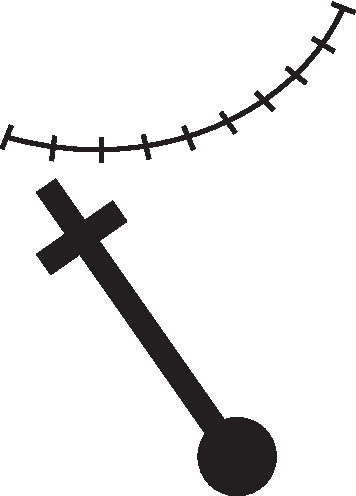
\includegraphics[width=0.1\textwidth]{images/35_15_06_50v1}
   \\\hspace{5mm}\textit{[Fig. 1]}
  }
per Magnetem\protect\index{Sachverzeichnis}{magnes} ad perpetuum motum\protect\index{Sachverzeichnis}{motus!perpetuus}, refert si quis possit efficere ut magnes\protect\index{Sachverzeichnis}{magnes} nunc habeat vires, nunc alio opposito \edtext{vel interposito}{\lemma{}\Afootnote{vel interposito \textit{ erg.} \textit{ L}}} non habeat, eum effecturum motum perennem\protect\index{Sachverzeichnis}{motus!perennis}, sed hoc neminem hactenus potuisse. Ego vero puto sic posse: \edtext{item ajunt si magneti alius obvertatur, eatenus amittet vires, ergo posset fieri, ut ab uno latere obvertatur}{\lemma{posse:}\Afootnote{ \textit{ (1) }\ si \textit{ (2) }\ ajunt ipsi magnetem\protect\index{Sachverzeichnis}{magnes|textit} armatum esse fortiorem inermi, non tamen pariete interposito aliquo, ergo si aliquid ei interponatur certo tempore per machinam, tunc trahet porro, non retrahet, quia ab uno latere interpositum est ab altero non est. \textit{ (3) }\ item [...] obvertatur \textit{ L }}}, et talia plura possunt practicari. Quare miror cur pater Kircher\protect\index{Namensregister}{\textso{Kircher} (Kircherus), Athanasius SJ 1602\textendash 1680} d. l. quaerat: quis hic?\edtext{}{\lemma{hic?}\Bfootnote{\textsc{A. Kircher}, \cite{00067}a.a.O., S.~243.}}
\pend 